\begin{figure}[t]
\centering
\subfigure[Bild]{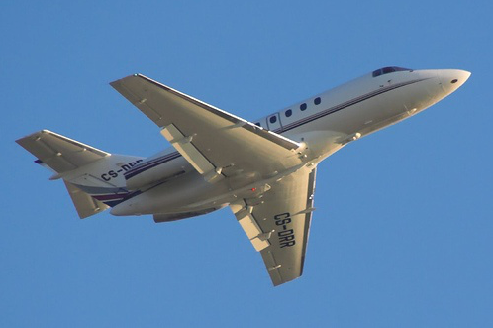
\includegraphics[scale=0.27]{bilder/flugzeug}}
\subfigure[Superpixel]{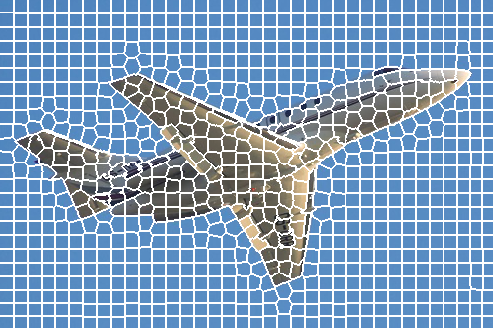
\includegraphics[scale=0.27]{bilder/flugzeug_slic}}
\subfigure[Graphrepräsentation]{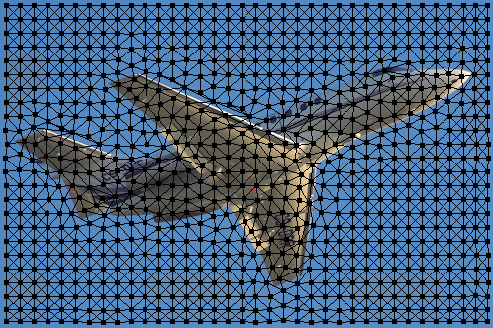
\includegraphics[scale=0.27]{bilder/flugzeug_slic_graph}}
\caption[Graphgenerierung aus einer Superpixelrepräsentation]{Illustration des Prozesses zur Graphgenerierung anhand einer Superpixelrepräsentation eines Bildes.
Ein Bild (a) wird dafür zuerst in eine Superpixelrepräsentation gebracht (b).
Die absoluten Zentren der Regionen bilden die Knotenpunkte des Graphen.
Benachbarte Regionen werden über eine Kante miteinander verbunden (c).}
\label{fig:superpixel_graph}
\end{figure}
